
¿Cuál es el perímetro del triángulo de la figura \ref{fig:peri_isos_02}?

% \begin{minipage}[t][][t]{0.3\textwidth}
\begin{figure}[H]
    \centering
    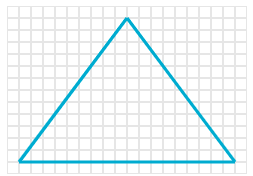
\includegraphics[width=0.2\textwidth]{../images/peri_isos_02.png}
    \caption{}
    \label{fig:peri_isos_02}
\end{figure}
% \end{minipage}\hfill
% \begin{minipage}[t][][t]{0.68\textwidth}
\begin{solutionbox}{16cm}
    \begin{minipage}{0.3\textwidth}
        \begin{figure}[H]
            \centering
            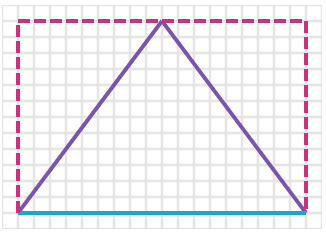
\includegraphics[width=0.6\linewidth]{../images/peri_isos_02a.png}
            \caption{}
            \label{fig:peri_isos_02a}
        \end{figure}
        \begin{figure}[H]
            \centering
            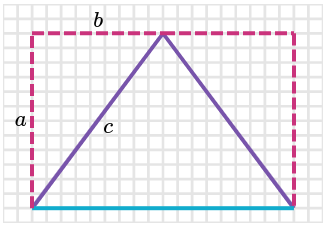
\includegraphics[width=0.6\linewidth]{../images/peri_isos_02b.png}
            \caption{}
            \label{fig:peri_isos_02b}
        \end{figure}
        \begin{figure}[H]
            \centering
            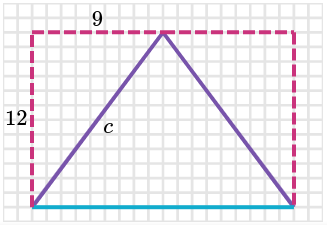
\includegraphics[width=0.6\linewidth]{../images/peri_isos_02c.png}
            \caption{}
            \label{fig:peri_isos_02c}
        \end{figure}
        \begin{figure}[H]
            \centering
            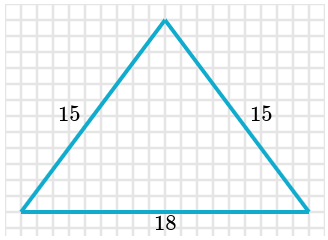
\includegraphics[width=0.6\linewidth]{../images/peri_isos_02d.png}
            \caption{}
            \label{fig:peri_isos_02d}
        \end{figure}
    \end{minipage}\hfill
    \begin{minipage}{0.65\textwidth}
        El perímetro es la distancia alrededor de una figura.
        Cada recta diagonal es la hipotenusa de un triángulo rectángulo (ver Figura \ref{fig:peri_isos_02a}).
        Podemos utilizar el teorema de Pitágoras para encontrar un lado faltante.
        La ecuación del teorema de Pitágoras es:
        \[c^2=a^2+b^2\]
        donde $a$ y $b$ son las longitudes de los catetos, y $c$ es la longitud de la hipotenusa.
        Etiquetemos la Figura del problema con $a$, $b$ y $c$ (ver Figura \ref{fig:peri_isos_02b}).
        Podemos contar los cuadrados para encontrar las longitudes de $a$ y $b$, y luego sustituir esos valores en el teorema de Pitágoras (ver Figura \ref{fig:peri_isos_02c}).
        \begin{align*}
            a^2+b^2  =c^2  & \text{\quad El teorema de Pitágoras}                          \\
            12^2+9^2  =c^2 & \text{\quad Sustituye las longitudes}                         \\
            144 +81 =x^2   & \text{\quad Evalua los cuadrados conocidos}                   \\
            225=x^2        & \text{\quad Sumando }                                         \\
            15=x           & \text{\quad Calculando la raíz en ambos lados de la ecuación} \\
        \end{align*}
        Ahora que conocemos la longitud de las diagonales, podemos encontrar la longitud del lado faltante para calcular el perímetro.
        Como el lado faltante es una línea horizontal (ver Figura \ref{fig:peri_isos_02d}), podemos contar los cuadrados para obtener su longitud.
        \[15+15+18=48\]
        El perímetro del triángulo es 48 unidades.
    \end{minipage}
\end{solutionbox}
% \end{minipage}
